\addtocontents{toc}{\protect\newpage}   % Start on new page in table of contents 
\chapter{User Manual}
This chapter describes the function and operation of the device, the system specifications and possible error scenarios with a potential cause of the problem. In addition, instructions are available for setting up the device and change the configuration.

\section{Configuration}
\subsection{System Setup}
After production, the blank \gls{esp32}-S2 must be programmed with the latest firmware. This can be achieved by following the steps in Section \ref{Firmware Update}. Next, the system configuration as well as the \acrshort{fms}-frame filter configuration must be loaded onto the root directory of the mass storage device. Figure\;\ref{fig:fleet-monitor-root-directory} shows how the file structure should look like when plugged in to a \acrshort{pc} via the \acrshort{usb}-interface.

\medskip
\begin{figure}[h!]
	\centering
	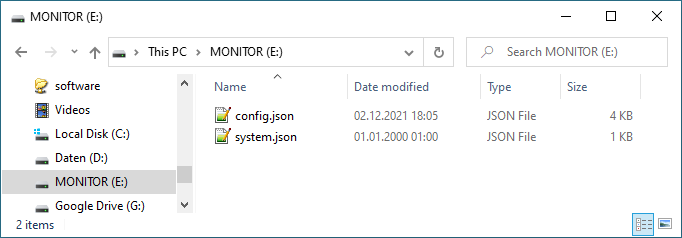
\includegraphics[width=13cm]{images/File_Explorer}
	\caption{Fleet-Monitor Root Directory}
	\label{fig:fleet-monitor-root-directory}
\end{figure}

Furthermore, parameters in the system configuration file must be adjusted to the needs of the overall setup. This contains setting the host \acrshort{ip} address and port number, as well as the \acrshort{ssid} and password if the device should connect over WiFi. Additional options can be defined, please refer to Section \ref{System Configuration} for more information.
\newpage

\subsection{Firmware Update} \label{Firmware Update}
\begin{wrapfigure}{r}{5.2cm}
\vspace{-0.6cm}
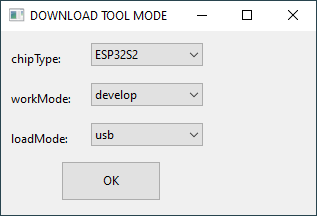
\includegraphics[width=5.2cm]{images/ESP32_Download_Mode}
\vspace{-0.4cm}
\caption{ESP32 Download Tool}
\label{fig:esp32-download-tool}
\end{wrapfigure} 
Espressif offers a firmware download tool for the \gls{esp32}-Family \cite{flash-download-tools}. When starting the application, the options in the dialog box should be set as shown in Figure \ref{fig:esp32-download-tool}. After pressing OK, the main window appears. 
To establish a connection to the \gls{esp32}-S2 over the \acrshort{usb}-interface, it has to be set into \acrshort{dfu}-Mode. This can be achieved by pressing the \textit{boot} button while resetting or power-cycling the device. If the device is already programmed with a firmware version that supports entering the \acrshort{dfu} mode by software, the \texttt{bootloader} flag can be set to \texttt{true} in the system configuration file as mentioned in Section \ref{System Configuration}.

The next step is to load the binary files at a specific location (offset as HEX index) in the flash memory. The first three files are called \texttt{bootloader\_qio\_40m.bin}, \texttt{partitions.bin} and \texttt{boot\_app0.bin}. These files are independent of the firmware and must not be changed. The fourth file called \texttt{firmware.bin} can be loaded directly from the build folder of the \acrshort{ide} (e.g. Visual Studio Code) and placed at offset \codeword{0x10000}. \\
In this case the following path is used: \texttt{FleetMonitor$\backslash$.pio$\backslash$build$\backslash$esp32s2dev}

Change the programming options of the download tool so that they exactly match Figure\;\ref{fig:esp32s2-download-tool-settings}. Now select the correct COM-Port and press the \texttt{START} button. It takes around 10\;seconds to upload the firmware. After updating, the device has to be reset and the new firmware gets executed. Note that this procedure does not touch the file system and therefore no data is being lost.

\begin{figure}[h!]
	\centering
	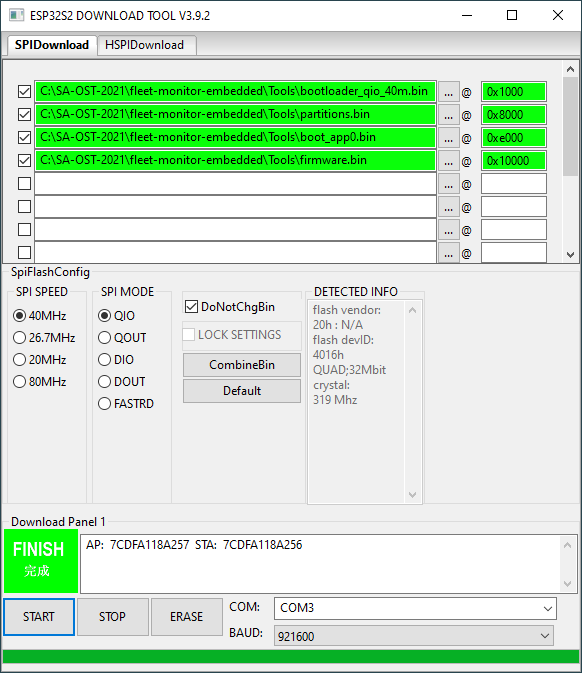
\includegraphics[width=9.2cm]{images/ESP32_Firmware_Settings}
	\caption{ESP32S2 Download Tool Settings}
	\label{fig:esp32s2-download-tool-settings}
\end{figure}
\newpage

\section{Specifications}
\begin{center}
    \begin{tabular}{p{6.4cm} p{6.4cm}}
    %\hline
    External Input Voltage          & 9\,V - 28\,V                      \\ %\hline
    Power Consumption               & 2.5\,W                            \\ %\hline
    Dimensions (L x W x D)          & 160 x 89 x 61\,mm                 \\ %\hline
    Weight                          & 350\,g                            \\ %\hline
    Water Resistance Rating         & IP67                              \\ %\hline
    Power Connector                 & M12 R/A F                         \\ %\hline
    Microprocessor                  & ESP32-S2                          \\ %\hline
    LAN-Interface                   & 10\,Base-T / 100\,Base-TX         \\ %\hline
    WLAN-Interface                  & 802,11b/g/n                       \\ %\hline
    USB-Interface                   & USB 2.0 (Device)                  \\ %\hline
    CAN-Interface                   & 250\,kbit/s (SAE J1939)           \\ %\hline
    
    \end{tabular}
\end{center}

\section{Device Status and Troubleshooting}


\subsection{LED Status}
The Fleet-Monitor uses two \acrshort{rgb} \acrshort{led}s to indicate the current status. Additionally there are two \acrshort{led}s located to the left of the RJ45 connector showing the link status and link activity.

\begin{center}
    \begin{tabular}{| p{6.4cm} | p{6.4cm} |} \hline
    \multicolumn{1}{|c|}{\textbf{Status LED}} & \multicolumn{1}{c|}{\textbf{Description}}   \\ \hline 
    White breathing                 & System is booting up                                  \\ \hline
    Blue breathing                  & System tries to connect to network                    \\ \hline
    Green                           & Connected to server over Ethernet                     \\ \hline
    Yellow                          & Connected to server over WiFi                         \\ \hline
    Magenta                         & Unable to establish server connection                 \\ \hline
    Red blinking                    & Unable to load configuration file                     \\ \hline
    
    \end{tabular}
\end{center}

\begin{center}
    \begin{tabular}{| p{6.4cm} | p{6.4cm} |} \hline
    \multicolumn{1}{|c|}{\textbf{CAN LED}} & \multicolumn{1}{c|}{\textbf{Description}}      \\ \hline 
    Off                             & Device is not receiving \acrshort{can} data           \\ \hline
    Green blinking                  & Device is receiving \acrshort{can} data               \\ \hline
    Red blinking                    & Error on physical interface                           \\ \hline
    \end{tabular}
\end{center}
\newpage

\subsection{Resolving Issues} \label{Resolving Issues}

\subsubsection{Status LED breathing white}
Normally this status clears within one or two breathing cycles. If the status does not clear the device is most likely in a boot loop. If this happens something is seriously wrong with the hard- or software. Refer to Section \ref{Hard Reset} for a resolution.

\subsubsection{Unable to connect to network}
The blue \acrshort{led} will breathe while the device is trying to establish a network connection. Connecting over WiFi or Ethernet can take up to one minute. The status is cleared as soon as a connection is received and an \acrshort{ip} address was assigned. If no connection can be established over an extended period of time the following things should be checked in order.

\textbf{Connecting over WiFi:}
\begin{enumerate}
  \item Make sure the device is not obstructed and close to the \acrlong{ap} in order to establish a connection. Metals, carbon fiber, and other \acrshort{rf} shielding materials should be kept away from the antenna of the \gls{esp32}.
  \item Make sure the \acrlong{ap} is password protected with \acrshort{wpa} or \acrshort{wpa}2. Both \acrshort{wep} and \acrshort{wpa}3 are not supported.
  \item Make sure the \acrlong{ap} name and password are set correctly in the system configuration. Please limit your passwords to \acrshort{ascii} characters, special Unicode characters are not allowed. Remember, the system automatically clears the password from the \texttt{system.json} file after a reboot but stores it locally.
  \item Make sure other devices like phones or computers can reach the \acrlong{ap}. If they are unable to, you may have a problem on the \acrshort{ap} side.
\end{enumerate}

\textbf{Connecting over Ethernet:}
\begin{enumerate}
  \item Make sure the \acrshort{led}s on the left side of the RJ45 connector are showing activity. If that is not the case check the following things.
  \begin{itemize}
      \item Make sure the \acrlong{ap} is powered on.
      \item Make sure the RJ45 cable is plugged in completely on both sides.
      \item Make sure the RJ45 cable is not faulty.
      \item Try connecting another device to the RJ45 cable and see if it receives a connection.
  \end{itemize}
  If all of these checks pass you may have a soft- or hardware issue. Refer to Section \ref{Hard Reset} for a resolution.
  \item Make sure the \acrlong{ap} is capable of \acrshort{dhcp}. The Fleet-Monitor gets the \acrshort{ip} address through the \acrlong{dhcp}. There is no support for static \acrshort{ip} addresses.
\end{enumerate}
\newpage

\subsubsection{Unable to establish server connection}\label{Unable to establish server connection}
If the status \acrshort{led} is not cleared after a short while, the Fleet-Monitor is unable to establish a connection to the server. The device is connected to an \acrshort{ap}, received an \acrshort{ip} address but the \acrshort{http} POST requests are unanswered or a bad status is returned. The following things should be checked to resolve this issue.

\begin{enumerate}
  \item Make sure the \acrshort{http} server is running and can respond to POST requests. The Fleet-Monitor is expecting to receive a response from the server with the status code of \texttt{200}. Otherwise, it will not clear the error.
  \item Make sure the \acrshort{ip} address and port are configured correctly in the system configuration file.
  \item Make sure to check if a request times out or an error code is returned from the server. The Fleet-Monitor will print the server response to the serial port. Section \ref{Serial Monitor} explains how to access the serial port.
\end{enumerate}

\subsubsection{Unable to load configuration file}
If the status \acrshort{led} is blinking red the device was unable to load the configuration file. 

A missing or corrupt file system is possible if the configuration can not be loaded locally.

To force manual reformatting of the file system, the \textit{boot} button must be pressed for 5 seconds while the device is in operation (not during a reset of the device).\\
\textbf{ATTENTION: THIS PROCEDURE WILL DELETE ALL FILES!}

In case the system is configured to load the file from the server you may need to refer to the error: Unable to establish server connection \ref{Unable to establish server connection}. The only difference is that these requests are done with \acrshort{http} GET instead of POST. Make sure your server can handle the requests to the Fleet-Monitor's specification.

\subsubsection{Device is not receiving CAN data}
In case the \acrshort{can} \acrshort{led} is turned off, the device is unable to receive data from the \acrshort{can} bus. You may want to try the following things.

\begin{enumerate}
  \item Make sure the \acrshort{can} termination is enabled on both ends of the bus.
  \item Make sure the \acrshort{can} data polarity is correct (CANH / CANL).
  \item Make sure the cable has the correct pin-out and no wires are damaged. 
  \item Make sure the \acrshort{fms} Gateway from the vehicle is transmitting data.
\end{enumerate}

\subsubsection{CAN Hardware Error}
In case the \acrshort{can} \acrshort{led} is blinking red, something went wrong in the initialization process of the \acrshort{can} interface. You may need to do a hard reset explained in Section \ref{Hard Reset}.

\newpage

\subsection{Serial Monitor} \label{Serial Monitor}
Diagnostics information is printed to the serial monitor to help the user debug an issue. Accessing the terminal can be done in just a few steps.

\begin{enumerate}
  \item Get a serial terminal tool for your computer. If you are running Windows, \mbox{\textit{TeraTerm}} is highly recommended. 
  \item Connect the Fleet-Monitor to your computer with a \acrshort{usb} cable.
  \item Locate the assigned serial port (e.g. using the \textit{Device Manager} on Windows).
  \item Run your serial terminal tool and connect to the open port. In \mbox{\textit{TeraTerm}}, under \textit{File {$\rightarrow$} New Connection} the serial port can be selected as shown in Figure \ref{fig:tera-connect}. Your port may vary. 
  \begin{figure}[h!]
	\centering
	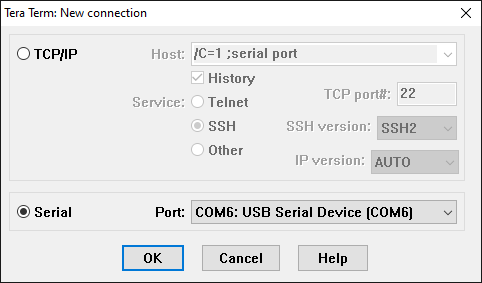
\includegraphics[width=9.2cm]{images/tera-connect}
	\caption{Open serial port through \mbox{\textit{TeraTerm}}}
	\label{fig:tera-connect}
\end{figure}
    \item Information is now being printed to the terminal and should look something like the example below.
    \bigskip
    \colorlet{mygray}{black!30}
    \colorlet{mygreen}{green!60!blue}
    \colorlet{mymauve}{red!60!blue}
    \begin{lstlisting}[backgroundcolor=\color{gray!10},  
                       basicstyle=\ttfamily,
                       columns=fullflexible,
                       breakatwhitespace=false,      
                       breaklines=true,                
                       captionpos=b,                    
                       commentstyle=\color{mygreen}, 
                       extendedchars=true,              
                       frame=single,                   
                       numbers=none,                
                       numbersep=5pt,                   
                       numberstyle=\color{blue}, 
                       rulecolor=\color{mygray},        
                       showspaces=false,
                       showstringspaces=false,
                       showtabs=false,                 
                       stepnumber=5,                  
                       stringstyle=\color{mymauve},    
                       tabsize=2,                      
                       title=\lstname,
                       frame=none,
                       xleftmargin = 1cm,
                       framexleftmargin = 1em]
    Connected over WiFi
    Loading config from server
    Status code: 200
    Config loading successful!
    \end{lstlisting}
\end{enumerate}

\subsection{Hard Reset} \label{Hard Reset}
If there is a serious issue with the device, the first action should be to reformat the file system and then upload the configuration files again. If this did not resolve the problem you may want to flash a known to be working firmware to the device. This is explained in Section \ref{Firmware Update}. If the issue persists, some parts of the hardware could be damaged and need to be replaced.
